%---------------------------------------------------------------------------
\svnidlong 
{$HeadURL: https://svn.fil.univ-lille1.fr/svn/sedoglav_PDC/trunk/Cours/03/03.tex $} 
{$LastChangedDate: 2012-09-14 14:32:35 +0200 (Fri, 14 Sep 2012) $} 
{$LastChangedRevision: 79 $} 
{$LastChangedBy: sedoglav $} 
\svnid{$Id: 03.tex 79 2012-09-14 12:32:35Z sedoglav $} 
% \slideheading{Plan de la s\'eance}%
% \begin{enumerate}
% \item Fonctions
%   \begin{itemize}
%   \item d\'efinition d'une fonction~: ANSI \& Kernighan et Ritchie
%   \item appel \`a une fonction
%   \item passage de param\`etres par valeur 
%   \end{itemize}
% \item Tableau
%   \begin{itemize}
%   \item d\'eclaration et initialisation
%   \item manipulations \'el\'ementaires
%   \end{itemize}
% \item Illustration le crible d'\'Eratosth\`ene
% \item Compilation s\'epar\'ee et make
% \end{enumerate}    
%------------------------------------------------------------------------------
\section{D\'efinition d'une fonction~: ANSI}
\begin{frame}[fragile]
  \alert{Syntaxe ANSI}~:
  {\it d\'{e}finition-de-fonction-ANSI} :
  \begin{center}
    \begin{tabular}[t]{l}
      {\it type-retour} \\
      {\it identificateur-de-fonction}
      \\
      {\tt (} \;
      {\it liste-de-param\`etres-typ\'es\/$_{option}$} \;
      {\tt )}
      \\
      {\tt \{} \\
      {\it liste-de-d\'{e}clarations-locales\/$_{\hspace{1mm}option}$}\\
      {\it liste-d'instructions}\\
      {\tt \}}
    \end{tabular}
  \end{center}
  \begin{overprint}
    \onslide<1>
    \alert{S\'emantique}~:
    \begin{itemize}
    \item {\it type-retour}~: type de la valeur retourn\'ee (quelconque),
    \item {\it liste-de-param\`etres-typ\'es\/$_{option}$}~:\\
      \quad liste des param\`etres formels avec leur type~;
    \item passage de param\`etres {\em uniquement} par valeur~;
    \item {\it liste-de-d\'{e}clarations-locales\/$_{\hspace{1mm}option}$}~:\\
      \quad d\'eclaration de variables {\em locales} \`a la fonction~;
    \item {\it liste-d'instructions}~: corps de la fonction.
    \end{itemize}
    \onslide<2>
    \alert{Une fonction retourne toujours une valeur}~: 
    \begin{itemize}
    \item le corps doit contenir au moins une
      instruction~: 
      \par
      \qquad \qquad{\tt return} \; {\it expression} \;{\tt ;}
     \par
      \hfill sinon le r\'esultat est ind\'etermin\'e~;
    \item {\it expression} qui doit \^etre de type {\it
        type-retour}~;
    \item cette instruction \'evalue {\it expression} qui sera la
      valeur de retour et rend le contr\^ole d'ex\'ecution \`a
      l'appelant.
  \end{itemize}
  \end{overprint}
  \index{D\'efinition!de fonctions}
  \index{D\'eclaration!de fonctions}
  \index{Fonctions!d\'efinition}
  \index{Passage de param\`etres}
  % \index{\verb?(,)?}
\end{frame}
%------------------------------------------------------------------------------
\begin{frame}[fragile]
  \frametitle{D\'efinition \`a la Kernighan et Ritchie}
  \begin{center}
  \alert{Syntaxe K\&R}~:     \begin{tabular}[t]{l}
      {\it type-retour} \; {\it identificateur-de-fonction} \\
      {\tt (} \; {\it liste-d'identificateurs\/$_{option}$} \; {\tt )}\\
      {\it liste-de-d\'{e}clarations\/$_{1 \hspace{1mm}option}$}\\
      \{ \\
      {\it liste-de-d\'{e}clarations\/$_{2 \hspace{1mm}option}$}\\
      {\it liste-d'instructions}\\
      \}
    \end{tabular}
  \end{center}
  \alert{S\'{e}mantique~: similaire \`a la norme ANSI}
  \begin{itemize}
  \item {\it liste-d'identificateurs\/$_{option}$}~: liste des
    param\`etres formels sans sp\'ecification de type~;
  \item {\it liste-de-d\'{e}clarations\/$_{1\hspace{1mm}option}$}~:\\
    \quad d\'eclaration des types des param\`etres formels~;
  \item les identificateurs doivent \^etre identiques dans \\
    \quad {\it liste-d'identificateurs} et
    {\it liste-de-d\'{e}clarations\/$_1$}~;
  \item si un param\`etre est omis dans {\it
      liste-de-d\'{e}clarations\/$_1$}~: \\
    \quad son type par d\'efaut est {\tt int}.
\end{itemize}
\end{frame}
%------------------------------------------------------------------------------
\begin{frame}[fragile]
    \frametitle{Comparaison ANSI et K\&R}
 Exemple de d\'efinition de fonction: norme ANSI
 \par\bigskip
\begin{verbatim}
   int sum_square(int i, int j) 
   {
     int resultat;
     resultat = (i * i) + (j * j);
     return resultat;
   }
\end{verbatim}
\par\bigskip
 Exemple de d\'efinition de fonction: norme K\&R
\par\bigskip
\begin{verbatim}
   int sum_square(i,j)
     int i,j;           
   {
     int resultat;  

     resultat = (i * i) + (j * j);
     return(resultat);
   }
\end{verbatim}

\index{D\'efinition!de fonctions}
\index{Fonctions!d\'efinition}
%\index{\verb?(,)?}
\end{frame}
%------------------------------------------------------------------------------
\begin{frame}[fragile]
  \frametitle{Remarques compl\'ementaires}
  \begin{itemize}
  \item on ne peut  pas d\'efinir des fonctions dans des fonctions~;
  \item {\tt return} est une instruction comme une autre~: \\
    \quad  ainsi, elle peut \^etre utilis\'ee plusieurs fois dans le corps d'une fonction
\begin{verbatim}
   int 
   max
   (int a, int b) 
   {
     if (a > b) return (a); else return(b);
   }
\end{verbatim}
  \item r\'ep\'etons que si la derni\`ere instruction ex\'ecut\'ee
    dans une fonction n'est pas un {\tt return}, le r\'esultat
    retourn\'e est ind\'etermin\'e.
  \end{itemize}
  Dans les transparents du cours, les accolades ouvrantes des bloc
  d'instructions ne sont pas sur une ligne ind\'ependante uniquement
  pour permettre la pr\'esentation. Ce n'est pas un exemple \`a
  suivre.
  \index{D\'efinition!de fonctions}
  \index{Fonctions!d\'efinition}
\end{frame}
%------------------------------------------------------------------------------
\section{Appel \`a une fonction}
\begin{frame}[fragile]
\frametitle{Appel \`a une fonction}
\begin{itemize}
\item Syntaxe de l'appel \`a une fonction~:
{\it expression-appel} :\\
\quad $\Rightarrow$  {\it identificateur-de-fonction} 
\, {\tt (} \; {\it liste-d'expressions} \;{\tt )}
\item S\'{e}mantique~:
  \begin{itemize}
    \item \'evaluation des expressions de {\it liste-d'expressions}~;
    \item l'ordre d'\'evaluation n'est pas fix\'e par la norme~;
    \item r\'esultats pass\'es en param\`etres effectifs \`a la fonction~;
    \item le passage se fait par {\em valeur}~;
    \item contr\^ole d'ex\'ecution pass\'e au d\'ebut de {\it
        identificateur-de-fonction}~;
    \item{\it expression-appel}: valeur retourn\'ee par la fonction~;  
  \end{itemize}
\item Exemples~:
\begin{verbatim}
   int a = 2 , b = 3, c, d ;
   d = sum_square(a,a*b) / 2; 
   c = max(a+1,b++); 
\end{verbatim}
\end{itemize}
\end{frame}
%------------------------------------------------------------------------------
\begin{frame}[fragile]
  \frametitle{Proc\'edures~: fonctions avec effet lat\'eral}
  \begin{itemize}
  \item C ne comporte pas de concept de proc\'edures~;
  \item Les fonctions peuvent r\'ealiser tous les effets lat\'eraux voulus~;
  \item En~C, une \textit{proc\'edure} est une fonction qui ne retourne
    aucune valeur (plut\^ot une valeur ind\'etermin\'ee)~;
  \item ``Valeur ind\'etermin\'ee'' a un type de base, le type {\tt void}~; 
  \item Il n'a pas de {\tt return} dans le corps d'une fonction de
    type de retour void (pour faire cours, d'une proc\'edure)~;
  \item Exemple d'appel de proc\'edure~:
\begin{verbatim}
#include<stdio.h>
void testzero(int j) {
	if(j) return ; /* provoque la sortie */
	printf("test positif") ; return ;
}
int main(void) {	
	testzero(0);
	return 0 ;
}
\end{verbatim}
  \end{itemize}
  \index{Appel d'une fonction/proc\'edure}
  \index{Fonctions!appel}
  \index{Proc\'edures}
\end{frame}
%------------------------------------------------------------------------------
\begin{frame}[fragile]
  \section{Passage de param\`etres par copie}%
  En~C, les param\`etres sont des variables comme les autres.
  \par
  Un passage d'information se fait par {\em copie} des param\`etres.
\begin{verbatim}
void fct(int bar){      int main(void){  
   bar++  ;                int foo = 4 ;     
   return ;                fct(foo++) ;    
}                          return foo ;  
                        }                
\end{verbatim}
  \`A chaque appel de fonction, de l'espace m\'emoire est cr\'e\'e pour
  les param\`etres et les variables locales (et d\'etruit apr\`es
  l'appel lors du retour \`a l'appelant).
 \begin{center}
   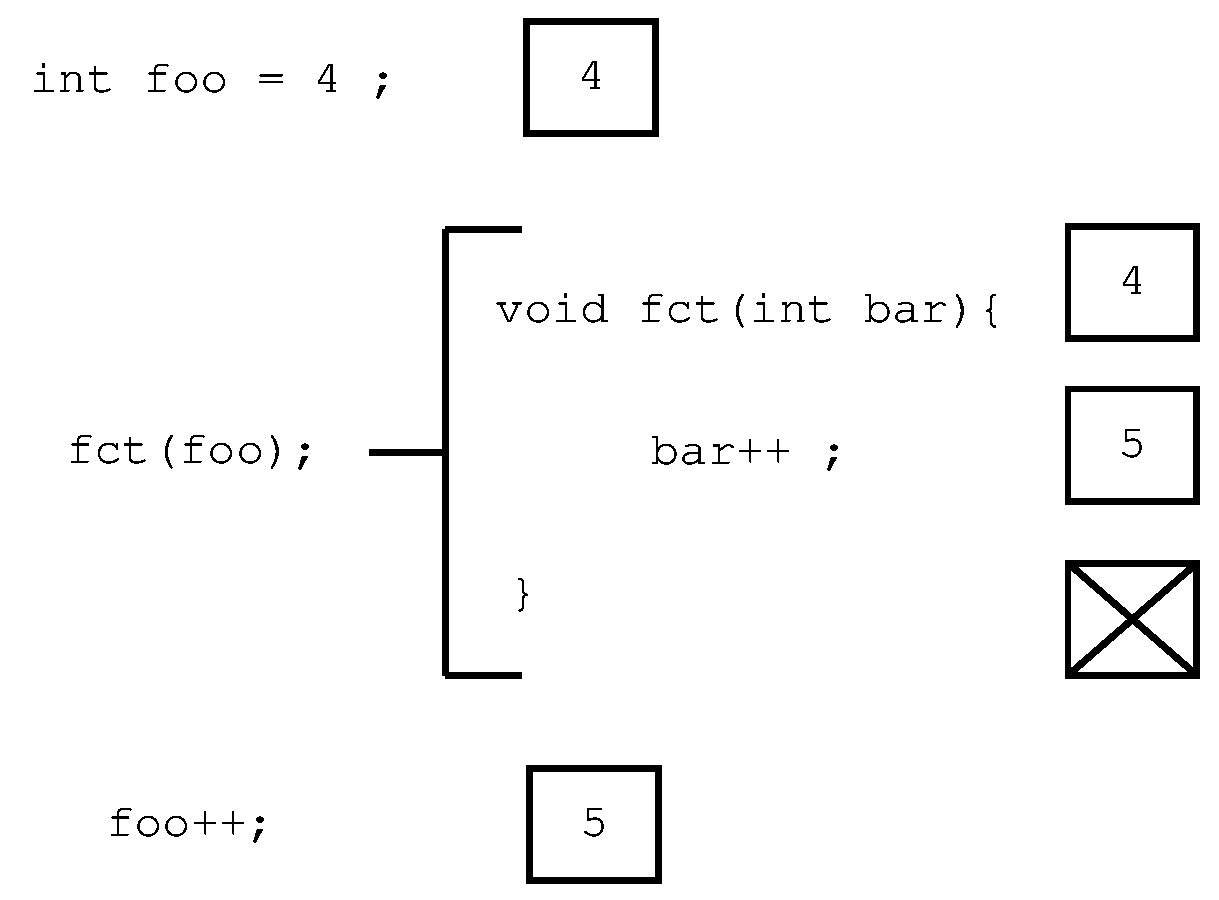
\includegraphics[scale=.2]{passPar}
 \end{center}
\end{frame}
%------------------------------------------------------------------------------
%\begin{frame}
%  \frametitle{De l'utilit\'e de faire de petit dessin}%
%\end{frame}
%------------------------------------------------------------------------------
\section{Les tableaux}
%------------------------------------------------------------------------------
\begin{frame}[fragile]
\frametitle{Les tableaux en C}
  En m\'emoire, un tableau est un bloc d'objets cons\'ecutifs de
  m\^eme type.
	\par\bigskip
  Sa d\'eclaration est~:
  \begin{itemize}
  \item similaire \`a une d\'eclaration de variable~;
  \item il faut indiquer le nombre d'\'el\'ements entre {\tt []}.
  \end{itemize}
	\par\bigskip
Quelques exemples~:
\begin{verbatim}
   char s[22]; /* s tableau de 22 caract\`eres */
   /* t1 tableau de 10 entiers longs et 
      t2 tableau de 20 entiers longs */
   long int t1[10], t2[20];
   #define N 100
   int tab[N/2];
\end{verbatim}
\end{frame}
%------------------------------------------------------------------------------
\begin{frame}[fragile]
  Points importants~:
  \begin{itemize}
  \item la taille d'un tableau est une constante
    \begin{bf}
      qui doit \^etre calculable \`a la compilation~:
    \end{bf}
\begin{verbatim}
char tab[] = "123" ;      .globl tab                   
                                .data                
int main(){                     .type   tab,@object  
                                .size   tab,4        
        return 0 ;        tab:                         
}                               .string "123"        
\end{verbatim}
  \item les indices dans un tableau commencent en 0~;
    \par\medskip
  \begin{bf}
    Les indices d'un tableau de taille {\tt N} vont de {\tt 0} \`a
    {\tt N-1}.
    \end{bf}
  \end{itemize}
\end{frame}
%------------------------------------------------------------------------------
\begin{frame}
  \frametitle{D\'efinition d'un tableau lors de sa d\'eclaration}
  L'initialisation d'un tableau se fait~:
  \begin{itemize}
  \item par des valeurs constantes plac\'ees entre {\tt \{\}}
    s\'epar\'ees par des virgules ({\tt ,})~;
  \item si il n'y a pas assez de valeurs~: l'espace m\'emoire restant est soit ind\'etermin\'e soit mis \`a~$0$~;
  \item Par exemple~: {\tt int t[4] = \{ 1, 2, 3, 4 \}}~;
  \item il n'y a pas de facteur de r\'ep\'etition.
  \end{itemize}
  \index{Tableaux!d\'eclaration}
  \index{Tableaux!initialisation}
\end{frame}
%------------------------------------------------------------------------------
\begin{frame}[fragile]
  \frametitle{Manipulations \'el\'ementaires sur les tableaux}
 Acc\`es \`a un \'el\'ement de tableau par op\'erateur d'indexation~;
 \begin{itemize}
 \item Syntaxe~: \\
   {\it expression} $\Leftarrow$ {\it identificateur-de-tableau} 
   {\tt [} {\it expression\/$_1$} {\tt ]}
 \item S\'{e}mantique~:
   \begin{itemize}
   \item {\it expression\/$_1$} d\'elivre une valeur enti\`ere~;
   \item {\it expression} d\'elivre l'\'el\'ement d'indice  {\it
       expression\/$_1$}~;
   \item {\it expression} peut \^etre une valeur de gauche comme
     dans l'exemple {\tt x = t[k]; t[i+j] = x;}.
   \end{itemize}
 \end{itemize}
 L'identificateur \verb?t? n'est pas une variable. Il est associ\'e
 \`a une adresse constante correspondant au d\'ebut de la m\'emoire
allou\'ee au tableau. En m\'emoire, on a les octets~:
 \begin{center}
   \begin{tabular}{c|c|c|c|c|c}
      & t  \\       \hline
      $\cdots$ & 1 & 2 & 3 & 4 &$\cdots$ \\ \hline
    \end{tabular}
  \end{center}
  Comparer~$2$ identificateurs de tableau revient \`a comparer~$2$
  adresses et non pas les objets stock\'es \`a ces adresses.  De
  m\^eme, affecter quelque chose \`a cet identificateur \verb?t = ...?
  n'a pas de sens.  \index{Tableaux!acc\`es \`a un \'el\'ement}
  \index{Op\'erateurs!indexation d'un tableau}
\end{frame}
%------------------------------------------------------------------------------
\begin{frame}[fragile]
  \section{Tableaux pass\'es en param\`etre d'une fonction}%
  \frametitle{Passage d'un tableau en param\`etre d'une fonction}%
  Puisque l'identificateur d'un tableau n'est pas une variable, quelle
  copie est faite lors du passage de param\`etre suivant~:
\begin{verbatim}
void fct(int tib[]){            int main(void){
   tib[0] = 1 ;                     int tab[2] = { 0, 1} ;
   return ;                         fct(tab) ;
}                                   return tab[0] ;   
                                }
\end{verbatim}
  C'est l'adresse qui est copi\'ee. Ceci implique que la fonction
  principale retourne~$1$ dans notre exemple.
  \par\medskip
  Dans \verb?fct?, \verb?tib[0]? fait r\'ef\'erence \`a la premi\`ere
  \textit{cellule m\'emoire} d\'efinie dans le tableau local \`a la
  fonction principale.
  \par\bigskip
  Nous \'etendrons ce principe (passage de param\`etre par adresse)
  aux autres types en utilisant la notion de pointeur.
\end{frame}
%------------------------------------------------------------------------------
\begin{frame}[fragile]
  \frametitle{Tableau bidimensionel}%
  Bien que stock\'es lin\'eairement, les tableaux peuvent \^etre
  d\'efinis comme multidimensionel~:
\begin{verbatim}
char tab[3][4]={"123","456","789"} ;  .file   "tableau2d.c"   
                                      .globl tab                   
int                                   .data                
main                                  .type   tab,@object  
(void)                                .size   tab,12       
{                                     tab:                         
   return 0 ;                         .string "123"        
}                                     .string "456"        
                                      .string "789"        
\end{verbatim}
  La s\'emantique est la m\^eme que pour le cas monodimensionnel~:
\begin{verbatim}
tab[3][0] = tab[3][0]++
\end{verbatim}
\end{frame}
% ------------------------------------------------------------------------------
\begin{frame}[fragile]
  \frametitle{Un petit coup d'oeil du cot\'e de l'assembleur}%
\begin{verbatim}
        .file   "tableau.c"          char tab[] = "123" ;
.globl tab                           unsigned int i =0 ; 
        .data                        int main(){            
        .type   tab,@object                         
        .size   tab,4                        i = tab ;   
tab:    .string "123"                        return 0 ;  
.globl i                             }                   
        .align 4
        .type   i,@object
        .size   i,4   /* Ce code compile en lan\c{c}ant un
i:      .long   0        avertissement~:
        .text            warning: assignment makes integer 
        .align 2         from pointer without a cast  */
.globl main                    
        .type   main,@function 
main:   ....... 
        movl    $tab, i   /* Nous verrons pourquoi lors de 
        movl    $0, %eax     l'\'etude des pointeurs     */
        .......
\end{verbatim}
\end{frame}
%------------------------------------------------------------------------------
%\begin{frame}
%  \section{Compl\'ement sur les tableaux}%
%
%\end{frame}
%------------------------------------------------------------------------------
\begin{frame}[fragile]
\section{Exemple de programme~: crible d'\'Eratosth\`ene}
\begin{verbatim}
   #include<stdio.h>
   #define IS_NON_PRIME 0
   #define IS_PRIME 1
   #define IS_CANDIDATE 2
   #define N 100

   int prem[N];

void init (void) 
{
     register int i;
     prem[0]=prem[1]=IS_NON_PRIME;
     for (i = 2; i < N; i = i + 1) prem[i] = IS_CANDIDATE;
     return ;
}

int min_is_candidate (void) 
{
     register int i = 0;
     while (prem[i] != IS_CANDIDATE) i = i + 1;
     return i;
}
\end{verbatim}
\end{frame}
%------------------------------------------------------------------------------
\begin{frame}[fragile]

\begin{verbatim}
void set_non_prime(int start) 
{
     register int i = start + 1;
     for (;i < N; i = i + 1)
       if (i % start == 0) prem[i]=IS_NON_PRIME;
     return ;
}

int main(void) 
{
     register int next_prime = 1, i;
      init();
     while (next_prime * next_prime < N) {
     next_prime=min_is_candidate();
     prem[next_prime]=IS_PRIME;
     set_non_prime(next_prime);
     }
     printf("Liste des nombres 
             premiers inf\\'erieurs \\`a %d\n", N);
     for (i = 0; i < N; i = i + 1)
       if (prem[i] != IS_NON_PRIME) printf("%d ", i);
     return 0 ;
}
\end{verbatim}
\index{Crible d'\'Eratosth\`ene}
\end{frame}
%------------------------------------------------------------------------------
\begin{frame}[fragile]
  \section{Compilation s\'epar\'ee et Make}%
  Nous allons reprendre l'exemple du crible d'\'Eratosth\`ene pour
  illustrer la notion de compilation s\'epar\'ee et l'utilitaire de
  gestion make associ\'e \`a cette notion.
  \par\medskip
  \textbf{Objectif}~: diviser un programme~C en plusieurs fichiers
  afin d'en faciliter la maintenance.
  \par\medskip
  Il faut prendre garde \`a g\'erer correctement les
  \textit{d\'ependances} entre les diff\'erents fichiers.
  \par\medskip
  Pour commencer, on peut regrouper les d\'efinitions de macro dans un
  fichier \texttt{eratosthene.h}~:
\begin{verbatim}
   #define IS_NON_PRIME 0
   #define IS_PRIME 1
   #define IS_CANDIDATE 2
   #define N 100
\end{verbatim}
  Un programme doit contenir une fonction principale (main).
\end{frame}
%------------------------------------------------------------------------------
\begin{frame}[fragile]
 La fonction principale \texttt{eratosMain.c} \\
 (permet entre autre de d\'eclarer les identificateurs)~:
\begin{verbatim}
#include <stdio.h>
#include "eratosthene.h"
void init (void) ;           /* le prototype des fonctions */
int min_is_candidate(void) ; /* utilis\'ees doit \^etre    */
void set_non_prime(int) ;    /* disponible                 */
int prem[N];      /* la variable globale est d\'efinie ici */
int main(void) {
     register int next_prime = 1, i;
     init();
     while (next_prime * next_prime < N) {
     next_prime=min_is_candidate();
     prem[next_prime]=IS_PRIME;
     set_non_prime(next_prime);
     }
     printf("Liste des nombres 
             premiers inf\\'erieurs \\`a %d\n", N);
     for (i = 0; i < N; i = i + 1) 
         if (prem[i] != IS_NON_PRIME) printf("%d ", i);
     return 0 ;
   }
\end{verbatim}
\end{frame}
%------------------------------------------------------------------------------
\begin{frame}[fragile]
\frametitle{Fichiers composant notre programme}
Il est possible d'obtenir un fichier objet associ\'e \`a ce code~:
\begin{verbatim}
% gcc -c eratosMain.c 
% ls
eratosMain.c eratosMain.o  eratosthene.h
\end{verbatim}
Puis, on peut par exemple faire un fichier par fonction~:
\begin{verbatim}
#include "eratosthene.h"
extern int prem [N] ; /* prototype de la variable globale */

void 
init 
(void) 
{ /* la d\'efinition de la fonction init */
   register int i;
   prem[0]=prem[1]=IS_NON_PRIME;
   for (i = 2; i < N; i = i + 1) prem[i] = IS_CANDIDATE;
   return ;
}
\end{verbatim}
\end{frame}
%------------------------------------------------------------------------------
\begin{frame}[fragile]
\frametitle{Obtention d'un ex\'ecutable}
Au final, on obtient
\begin{verbatim}
% gcc -c eratosInit.c 
% ls
eratosInit.c  eratosMain.c  eratosMin.c  eratosSet.c  
eratosInit.o  eratosMain.o  eratosMin.o  eratosSet.o 
eratosthene.h
\end{verbatim}
Pour conclure, on fait l'\'edition de lien de ces fichiers objets~:
\begin{verbatim}
% gcc -o executable eratos*.o
%  executable 
Liste des nombres premiers inf\'erieurs \`a 100
2 3 5 7 11 13 17 19 23 29 31 37 41 43 47 53 59 
61 67 71 73 79 83 89 97 
\end{verbatim}
\end{frame}
%------------------------------------------------------------------------------
\begin{frame}
\frametitle{Arbre de d\'ependances}
Les op\'erations pr\'ec\'edentes sont mod\'elis\'ees par
l'arbre de d\'ependances~: 
\par\bigskip
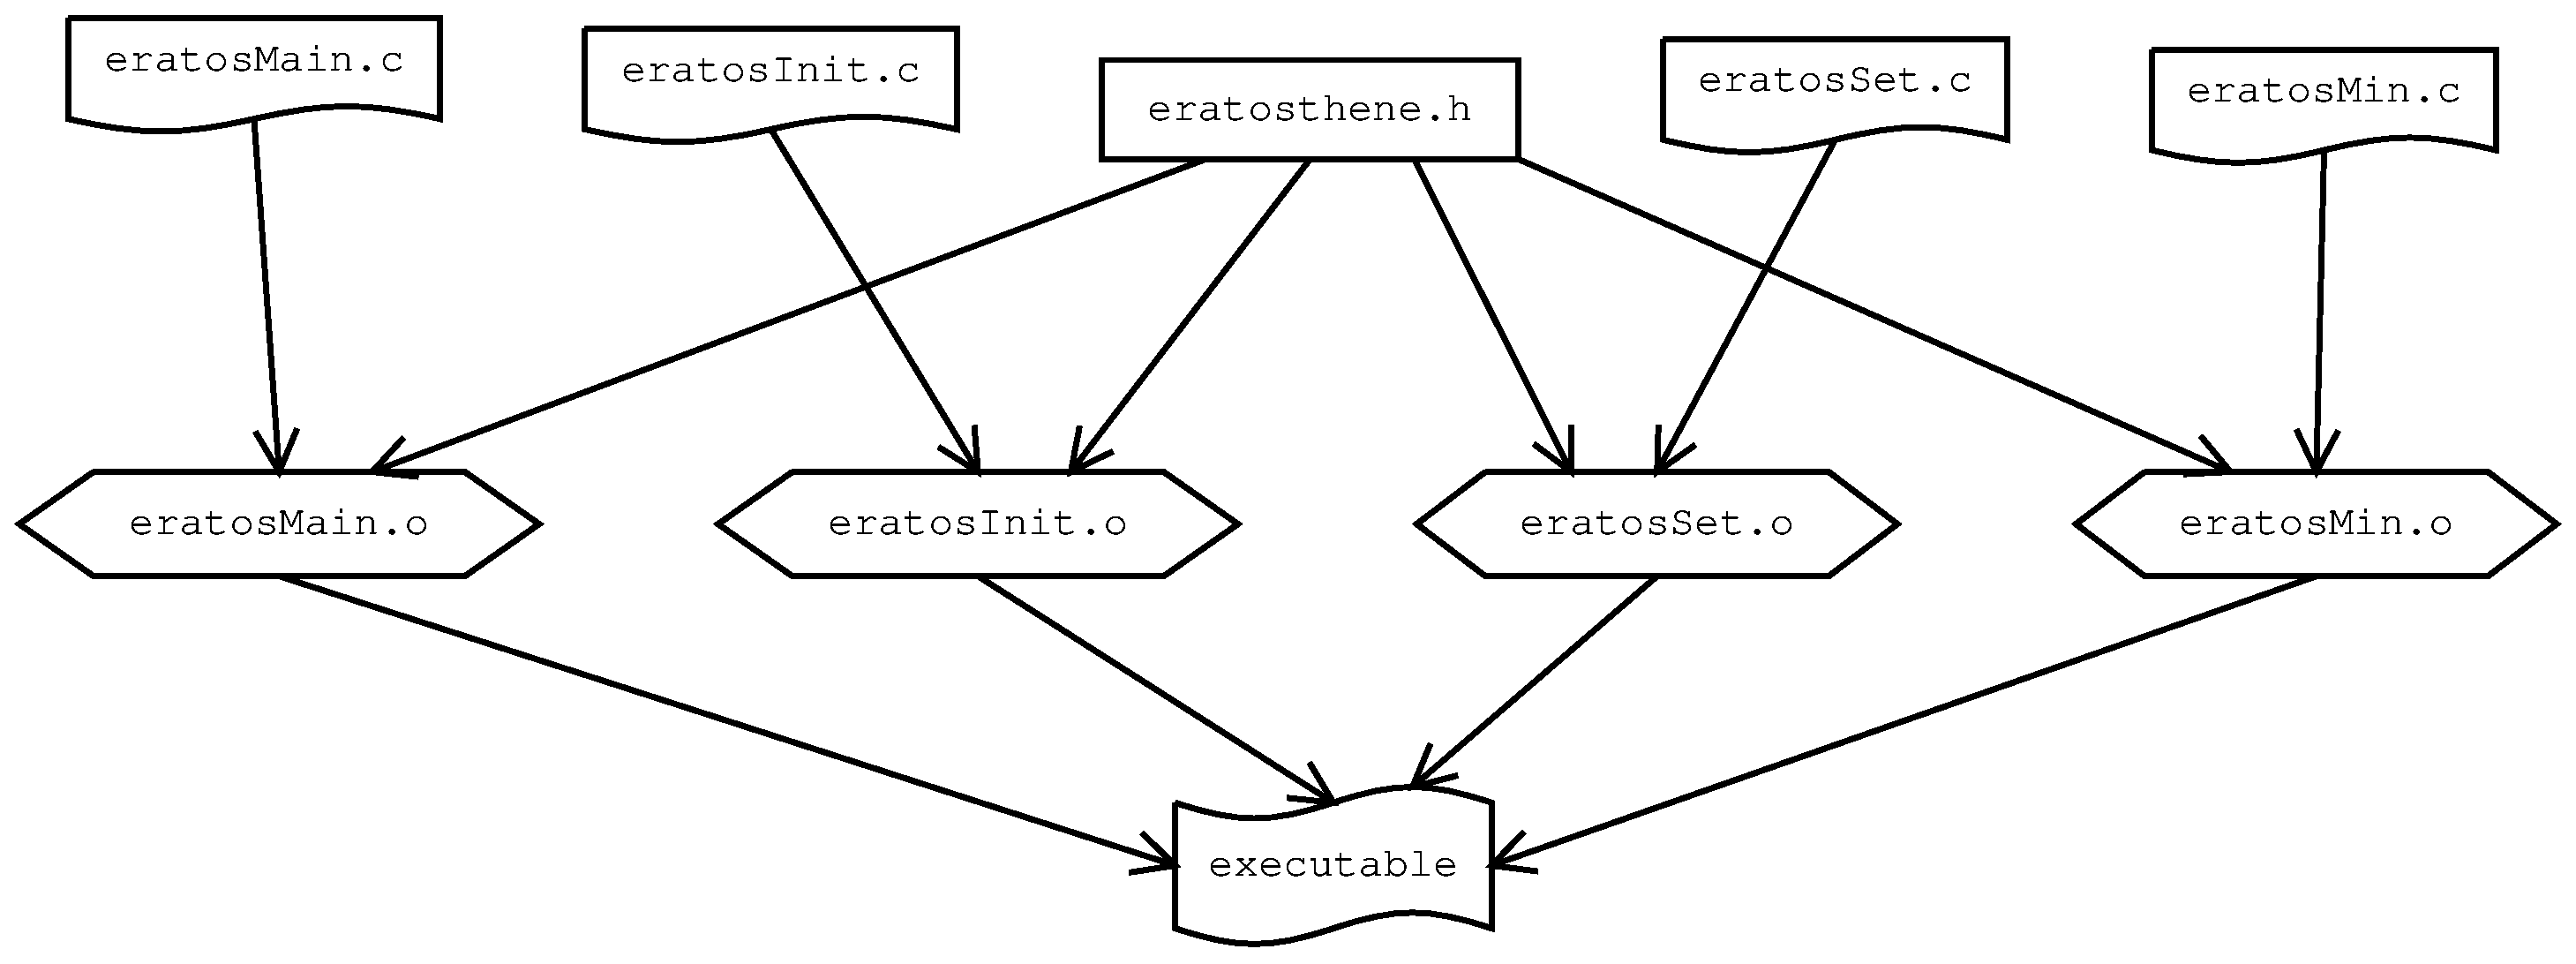
\includegraphics[scale=.2]{arbre}
\end{frame}
%------------------------------------------------------------------------------
\begin{frame}[fragile]
  \frametitle{Utilitaire {\tt make}~: syntaxe}%
  Pour les projets importants (le code source de Linux est constitu\'e
  de~$921$ fichiers), il faut automatiser les t\^aches.
  \par\medskip
  Automatisation de la compilation~:
  \begin{itemize}
  \item Maintenance, mise \`a jour et r\'eg\'en\'eration de fichiers
    d\'ependants~;
  \item Sources $\rightarrow$ ex\'ecutables~;
  \item Recompilation quand n\'ecessaire (dates)~; 
  \item Fichier de r\`egles de d\'erivation (code l'arbre de d\'ependances)\\
    \hspace*{10mm} {\tt Makefile} ou {\tt makefile}.
  \end{itemize}   
\end{frame}
%------------------------------------------------------------------------------
\begin{frame}[fragile]
Format d'une r\`egle~: quoi, pourquoi, comment.
\begin{itemize}
\item syntaxe~:
  \hspace*{10mm} {\it target}: {\it dependencies}\\
\hspace*{25mm} (tabulation){\it commands}
  \item\alert{quoi} ({\it target}) objectif, g\'en\'eralement un fichier~;
  \item\alert{pourquoi} ({\it dependencies}) liste des
    fichiers/cibles dont d\'epend {\it target}~;
  \item\alert{comment} ({\it commands}) commandes \`a ex\'ecuter pour r\'ealiser   
    {\it target}~;
\end{itemize}
On peut n'ex\'ecuter qu'une \textit{partie} de l'arbre~: \verb?%make target?
 \par
 Exemple (makefile pour un programme~C)
\begin{verbatim}
.PHONY:clean
executable: f1.o f2.o
        gcc -o executable f1.o f2.o
f1.o: f1.c fichier.h
        gcc -c f1.c
f2.o: f2.c fichier.h
        gcc -c f2.c
clean:
        rm -f *~ *.o executable
\end{verbatim}
\end{frame}
%------------------------------------------------------------------------------
%\begin{frame}
%  \frametitle{Utilitaire {\tt make}~: un exemple}
%\end{frame}
%------------------------------------------------------------------------------
\begin{frame}[fragile]
  \frametitle{Utilitaire {\tt make}~: notre exemple}
Dans notre cas, on peut \'ecrire le Makefile suivant~:
\begin{verbatim}
OPTIONS = -Wall -ansi -pedantic
OBJETS = eratosMain.o eratosMin.o eratosSet.o eratosInit.o

executable: $(OBJETS)
        gcc $(OPTIONS) -o executable $(OBJETS)

eratosMain.o: eratosMain.c eratosthene.h
        gcc $(OPTIONS) -c eratosMain.c

eratosMin.o: eratosMin.c eratosthene.h
        gcc $(OPTIONS) -c eratosMin.c

eratosSet.o: eratosSet.c eratosthene.h
        gcc $(OPTIONS) -c eratosSet.c

eratosInit.o: eratosInit.c eratosthene.h
        gcc $(OPTIONS) -c eratosInit.c
\end{verbatim}
\end{frame}
%------------------------------------------------------------------------------
\begin{frame}[fragile]
  \frametitle{Algorithme et  macros de make}%
\begin{itemize}
      \item Pour chaque cible 
        \begin{itemize}
          \item V\'erifier les d\'ependances
            \begin{itemize}
              \item [$\rightarrow$] R\'ecursion
              \item [$\rightarrow$] Date des fichiers de base
            \end{itemize}
          \item Si modification
            \begin{description}
              \item [\textnormal{alors} $\rightarrow$] Lancer les commandes 
              \item [\textnormal{sinon} $\rightarrow$] Fichier \`a jour
            \end{description}
        \end{itemize}
    \end{itemize}
    \par\bigskip
  \begin{itemize}
  \item[\$@] repr\'esente le nom complet de la cible courante~;
  \item[\$?] repr\'esente les d\'ependances plus r\'ecentes que la cible~;
  \item[\$$<$] repr\'esente le nom de la premi\`ere d\'ependance~;
  \item[\$\^{}] repr\'esente la liste de toutes les d\'ependances~;
  \end{itemize}
  On peut d\'efinir ses propres macros~:
\begin{verbatim}
REP = /etc/ /bin/ /usr/bin/
\end{verbatim}
\end{frame}
%------------------------------------------------------------------------------
\begin{frame}[fragile]
  \section{Ex\'ecution pas \`a pas dans l'environnement gnu debugger}%
\frametitle{Le d\'evermineur \texttt{gdb}}%
L'environnement \texttt{gdb} permet d'ex\'ecuter des programmes pas
\`a pas   et d'examiner  la   m\'emoire du processus en cours.

Pour utiliser gdb, l'ex\'ecutable doit avoir \'et\'e compil\'e avec l'option -g.

On l'utilise dans un shell en 
indiquant le fichier \`a examiner~:
\begin{verbatim}
% gdb executable
GNU gdb 5.3-22mdk (Mandrake Linux)
...... etc...................
This GDB was configured as "i586-mandrake-linux-gnu"...
(gdb) 
\end{verbatim}
Ce programme propose une aide en ligne~:
\begin{verbatim}
(gdb) help help
Print list of commands.
(gdb) help quit
Exit gdb.
\end{verbatim}
\end{frame}
%------------------------------------------------------------------------------
\begin{frame}[fragile]
  \frametitle{Ex\'ecution et examen du code source}%
Le programme consid\'er\'e peut \^etre ex\'ecut\'e dans l'environnement
\texttt{gdb}~:
\begin{verbatim}
(gdb) run
Starting program: /home/..../executable 
Liste des nombres premiers inf\'erieurs \`a 100
2 3 5 7 11 13 17 19 23 29 31 37 41 43 47 53 59 
61 67 71 73 79 83 89 97 
Program exited normally.
(gdb) 
\end{verbatim}
Lorsque le code source de l'ex\'ecutable est disponible la commande
\texttt{list} permet d'afficher le code source avec chacune de ces
lignes num\'erot\'ees. Dans notre cas~:
\begin{verbatim}
(gdb) list
1       #include <stdio.h>
2       #include "eratosthene.h"
3       
4       void init (void) ;
(gdb) 
\end{verbatim}
\end{frame}
%------------------------------------------------------------------------------
\begin{frame}[fragile]
  \frametitle{Placer des points d'arr\^et}%
La commande \texttt{break} permet de placer un point d'arr\^et sur une
instruction    du programme source   de   mani\`ere \`a  ce qu'\`a  la
procha\^\i{}ne ex\'ecution du programme dans \texttt{gdb}, l'invite du
d\'evermineur  soit     disponible    avant l'ex\'ecution     de cette
instruction.
\par 
Une instruction du programme source peut \^etre rep\'er\'ee par le
num\'ero de ligne correspondant ou par un identificateur~:
\begin{verbatim}
(gdb) break 10
Breakpoint 1 at 0x8048353: file eratosMain.c, line 10.
(gdb) break min_is_candidate
Breakpoint 2 at 0x80483f2: file eratosMin.c, line 4.
\end{verbatim}
permet de placer deux points d'arr\^ets aux endroits sp\'ecifi\'es. la commande
\texttt{info} fournit la liste des points d'arr\^ets~:
\begin{verbatim}
(gdb) info break
Num Type       Disp Enb Address    What
1   breakpoint keep y   0x08048353 in main at eratosMain.c:10
2   breakpoint keep y   0x080483f2 in min_is_candidate at ..
\end{verbatim}
\end{frame}
%------------------------------------------------------------------------------
\begin{frame}[fragile]
  \frametitle{Ex\'ecution pas \`a pas}%
  Une fois ceci fait, ex\'ecutons notre programme dans \texttt{gdb}~:
\begin{verbatim}
Starting program: /home/.../executable 
Breakpoint 1, main () at eratosMain.c:10
10           init();
(gdb) 
\end{verbatim}
  Pour provoquer l'appel \texttt{init()}, utilisons la commande
  \texttt{next}~:
\begin{verbatim}
(gdb) next
11           while (next_prime * next_prime < N) {
\end{verbatim}
  On peut ex\'ecuter les instructions associ\'ees
\begin{verbatim}
(gdb) step
init () at eratosInit.c:7
7         prem[0]=prem[1]=IS_PRIME;
\end{verbatim}
Pour ex\'ecuter les instructions jusqu'au prochain point
d'arr\^et
\begin{verbatim}
(gdb) continue
Continuing. Breakpoint 2, min_is_candidate () at eratosMin.c:4
4            register int i = 0;
\end{verbatim}
\end{frame}
%------------------------------------------------------------------------------
\begin{frame}[fragile]
  \frametitle{Affichage du contenu des variables et de la m\'emoire}
Pour  afficher  le contenu  d'une variable, il suffit d'utiliser print
\begin{verbatim}
(gdb) print prem
$3 = {0, 0, 1, 2, 0, 2, 0, 2, 0, 2, 0, 2, 0, 2, 0,.. etc..
  0, 2, 0, 2, 0, 2, 0, 2, 0, 2, 0, 2, 0, 2, 0, 2}
(gdb) 
\end{verbatim}
On peut provoquer l'affichage \`a chaque arr\^et avec display et le formatter avec printf
\begin{verbatim}
(gdb) printf "%x\n",prem[1]
1
\end{verbatim}
  Plus g\'en\'eralement, on obtient l'affichage d'une
  zone m\'emoire gr\^ace \`a la commande~:
\begin{verbatim}
(gdb) x /4xw 0xbffff6a4
0xbffff6a4: 0x00000064 0xbffff6b8 0x0804836b 0x4014cf50
\end{verbatim}
\end{frame}
%------------------------------------------------------------------------------
\begin{frame}[fragile]
  \frametitle{Quelques remarques~: gdb est un outils tr\`es puissant}%
  Remarquez qu'\`a l'entr\'ee d'une fonction, les param\`etres sont indiqu\'es~:
\begin{verbatim}
(gdb) contenu
Continuing.
Breakpoint 1, set_non_prime (start=3) at eratosSet.c:5
5            register int i = start + 1;
\end{verbatim}
  On peut modifier les valeurs des variables en cours d'ex\'ecution~:
\begin{verbatim}
(gdb) set variable start = 0xb 
(gdb) print start
$15 = 11
\end{verbatim}
  Il est possible de tracer l'ex\'ecution, de l'interrompre lors
  d'\'ev\'enements pr\'ed\'efinis, etc.

  Pour plus d'information, utilisez l'aide en ligne de gdb. 
\end{frame}
%------------------------------------------------------------------------------
\end{document}
%------------------------------------------------------------------------------
% Mod\`ele
%------------------------------------------------------------------------------
\begin{frame}
  \section{}%
\end{frame}
%------------------------------------------------------------------------------
